\begin{frame}{有效过程及初态条件}
  \small
  \begin{columns}[T,onlytextwidth]
    \begin{column}{0.49\textwidth}
      \vspace{2em}

      \hspace*{-0.30\linewidth}%
      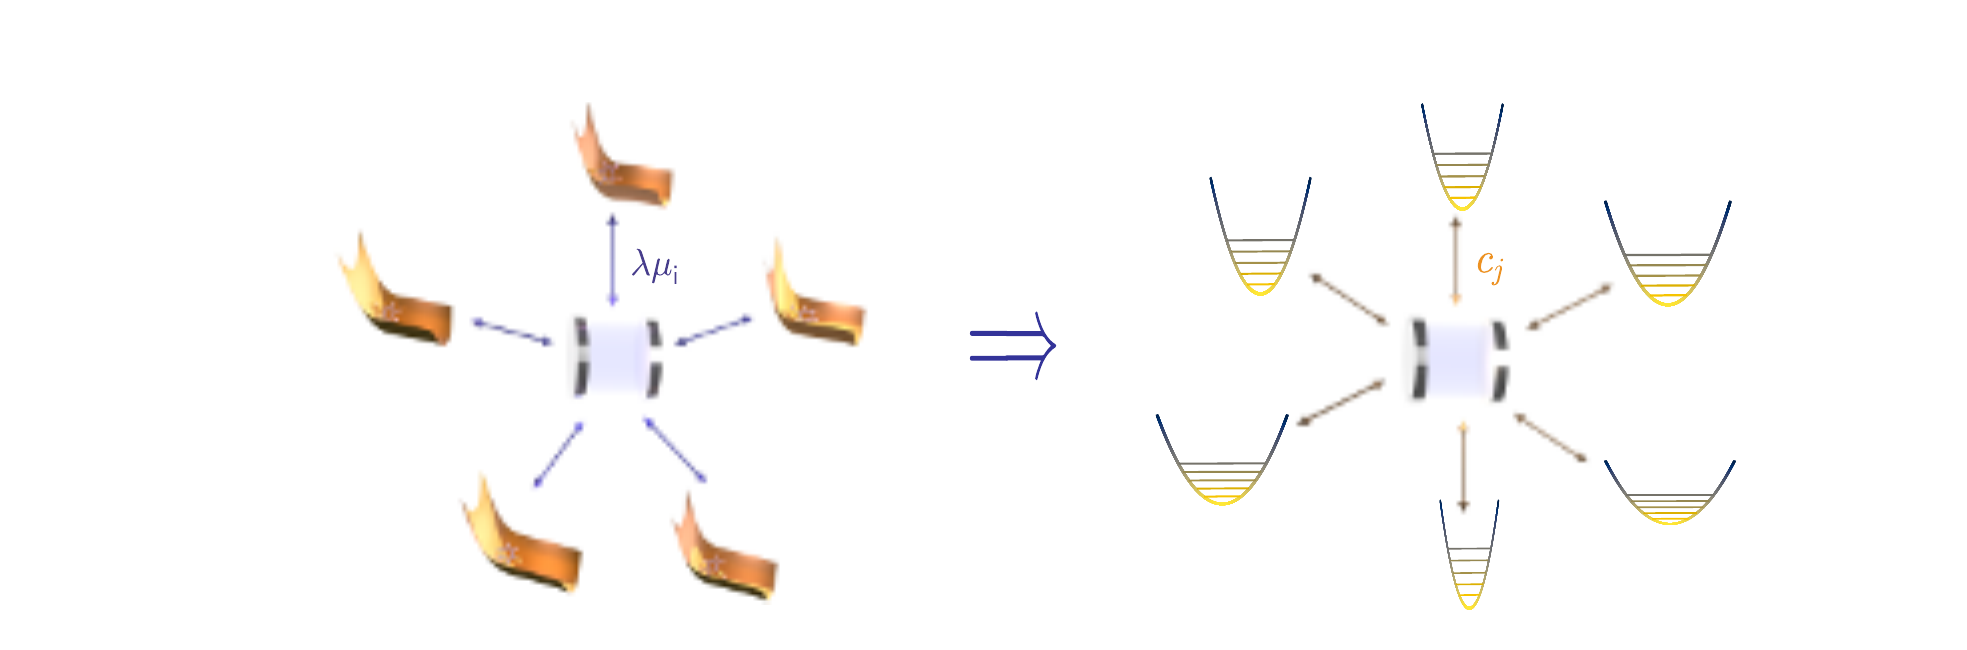
\includegraphics[width=1.5\linewidth,keepaspectratio]
        {figures/jcp_fig1_original.png}

    \end{column}
    \begin{column}{0.47\textwidth}
      \footnotesize

      将单模腔光子视为系统，分子系综视为环境。
      首先要求初态满足

      \[
        \rho(t_{\mathrm{in}})
        =
        \rho_{\mathrm{ph}}\otimes\rho_{\mathrm{mol}}
        =
        \rho_{\mathrm{ph}}\otimes
        \sum_y p_y|y\rangle\langle y|.
      \]

      {\color{gray}\hfill JCP Eq.~(6)}

      初始光与物质无关联；$\rho_{\mathrm{mol}}$ 是
      $H_{\mathrm{mol}}$ 的平稳态，不要求热平衡。

      \vspace{0.7em}

    \end{column}
  \end{columns}

  \papersource{Yuen-Zhou \& Koner,
  J. Chem. Phys. 160, 154107 (2024), Fig.~1.}
\end{frame}

\begin{frame}{分子系综作为腔光子的有效环境}

  \footnotesize
  \setlength{\abovedisplayskip}{4pt}
  \setlength{\belowdisplayskip}{4pt}

  \vspace*{0.4em}
  腔通过分子系综总偶极与分子环境耦合。
  {\fontsize{10.95}{13}\selectfont
  \[
    \begin{aligned}
      \hat\mu
        &=\sum_{i=1}^{N}\hat\mu_i,\\[0.3em]
      C_2(t)
        &=|\hbar\lambda|^2
          \langle\hat\mu(t)\hat\mu(0)\rangle\\
        &=|\hbar\lambda|^2\sum_i
          \langle\hat\mu_i(t)\hat\mu_i(0)\rangle.
    \end{aligned}
  \]}

  \vspace{0.6em}
  $C_2(t)$ 描述 $t=0$ 的偶极涨落经过时间 $t$ 后仍保留多少相关性。

  \vspace{0.8em}
  在 $N\to\infty$ 条件下，可用一个产生相同两时刻偶极关联的
  谐振子环境替代原复杂分子环境。
  {\fontsize{10.95}{13}\selectfont
  \[
    C_2^{\mathrm{eff}}(t)=C_2(t).
  \]}

  \papersource{JCP 160, 154107 (2024), Sec.~II, Eqs.~(13)--(14) 及 Eq.~(18) 。}

\end{frame}

\begin{frame}{谐振子环境的两时刻关联与有效谱密度}

  \footnotesize
  \setlength{\abovedisplayskip}{3pt}
  \setlength{\belowdisplayskip}{3pt}

  \vspace*{0.4em}
  等效谐振子环境由一组独立模式组成：
  {\fontsize{10.95}{13}\selectfont
  \[
    H_{\mathrm{mol}}^{\mathrm{eff}}
      =\sum\nolimits_j\hbar\omega_j b_j^\dagger b_j .
  \]}

  其谱密度定义为
  {\fontsize{10.95}{13}\selectfont
  \[
    J^{\mathrm{eff}}(\omega)
      \equiv\Theta(\omega)\pi\hbar
      \sum\nolimits_j|\bar c_j|^2\delta(\omega-\omega_j).
  \]}
  $J^{\mathrm{eff}}(\omega)$ 描述谐振子环境
  在不同频率处与腔模的耦合强度。

  \vspace{0.5em}
  对于线性谐振子环境，谱密度、模式布居和两时刻关联之间的关系是已知的。
  利用上一页的匹配条件 $C_2^{\mathrm{eff}}(t)=C_2(t)$，
  并结合正、负频率关系消去有效模式的布居信息，
  可得到 JCP Eq.~(18)：
  {\fontsize{10.95}{13}\selectfont
  \[
    J^{\mathrm{eff}}(\omega)
      =\frac{\ii\Theta(\omega)}{\hbar}
        \int_{-\infty}^{\infty}C_2(t)\sin(\omega t)\,dt.
  \]}

  因此真实分子的 $C_2(t)$ 已经足以确定
  等效谐振子环境的频率与耦合强度分布。

  \papersource{JCP 160, 154107 (2024), Eqs.~(8), (11), (13), (18).}

\end{frame}

\begin{frame}{有效谱密度由分子线性极化率给出}

  \scriptsize
  \setlength{\abovedisplayskip}{1pt}
  \setlength{\belowdisplayskip}{1pt}

  \vspace*{0.15em}
  {\fontsize{10}{12}\selectfont
  \[
    C_2(t)
    =\lim_{\gamma\to0^+}\sum\nolimits_{y,z}p_y
      |\hbar\lambda\langle z|\hat\mu|y\rangle|^2
      e^{-\ii(\omega_{zy}-\ii\gamma/2)t}.
  \]}
  将真实分子的两时刻偶极关联在 $H_{\mathrm{mol}}$ 本征态中展开：
  它是所有允许分子跃迁的叠加，
  每一项由跃迁频率、跃迁偶极和初态布居决定。

  \vspace{0.1em}
  将上述 $C_2(t)$ 代入上一页 Eq.~(18)，得到
  {\fontsize{10}{12}\selectfont
  \[
    J^{\mathrm{eff}}(\omega)
    =\Theta(\omega)\pi\hbar\sum\nolimits_{y,z}
      (p_y-p_z)|\lambda\langle z|\hat\mu|y\rangle|^2
      \delta(\omega_{zy}-\omega).
  \]}

  同一组分子跃迁也决定线性极化率。
  论文将其写成本征态谱表示（JCP Eq.~21b）：
  {\fontsize{10}{12}\selectfont
  \[
    \chi(\omega)
    =-\lim_{\gamma\to0^+}\sum\nolimits_{y,z}(p_y-p_z)
      \frac{|\lambda\langle z|\hat\mu|y\rangle|^2}
      {\omega-\omega_{zy}+\ii\gamma/2}.
  \]}

  $\operatorname{Im}\chi(\omega)$ 给出这组允许跃迁的吸收部分，
  因此论文 Eq.~(20) 得到
  {\fontsize{10}{12}\selectfont
  \[
    J^{\mathrm{eff}}(\omega)
    =\Theta(\omega)\hbar\,\operatorname{Im}\chi(\omega).
  \]}
  等效谐振子环境在各频率处需要多强地耦合，
  恰好由真实分子在这些频率处的吸收响应决定。

  \papersource{JCP 160, 154107 (2024), Eqs.~(18)--(21).}

\end{frame}

\begin{frame}{$N\to\infty$ 下：弱 probe 读取微腔线性光谱}

  \label{frame:cavity-response}

  \footnotesize
  \setlength{\abovedisplayskip}{2pt}
  \setlength{\belowdisplayskip}{2pt}

  $\omega_{\mathrm{ph}}$ 是固定的裸腔共振频率，
  裸分子系综对 probe 的线性响应由 $\chi(\omega)$ 给出。
  标准输入--输出理论将腔内线性响应转换为透射、反射和吸收光谱：

  \[
    T(\omega)
    =
    \frac{\kappa_L\kappa_R}
    {\left|
      \physmark{Plum}{p14det}{\omega-\omega_{\mathrm{ph}}}
      +
      \physmark{Bittersweet}{p14loss}{\ii\kappa/2}
      +
      \physmark{NavyBlue}{p14chi}{\chi(\omega)}
    \right|^2}.
  \]

  \begin{tikzpicture}[
      overlay,
      remember picture,
      >=stealth,
      nodes={align=center,inner ysep=1pt},
      <-
    ]

    \path (p14det.south) ++ (-1.4,-1.0em)
      node[anchor=north,color=Plum!85] (p14dettext)
      {\textsf{\footnotesize probe--裸腔失谐}};
    \draw[color=Plum]
      (p14det.south) |- (p14dettext.north east);

    \path (p14loss.south) ++ (0,-1.0em)
      node[anchor=north,color=Bittersweet!85] (p14losstext)
      {\textsf{\footnotesize 腔光子损耗}};
    \draw[color=Bittersweet]
      (p14loss.south) -- (p14losstext.north);

    \path (p14chi.south) ++ (1.4,-1.0em)
      node[anchor=north,color=NavyBlue!85] (p14chitext)
      {\textsf{\footnotesize 分子线性响应}};
    \draw[color=NavyBlue]
      (p14chi.south) |- (p14chitext.north west);

  \end{tikzpicture}

  \vspace{2.2em}

  \[
    A(\omega)
    =
    \frac{2\kappa_L\operatorname{Im}\chi(\omega)}
    {|\omega-\omega_{\mathrm{ph}}+\ii\kappa/2+\chi(\omega)|^2},
    \qquad
    R(\omega)=1-T(\omega)-A(\omega).
  \]

\vspace{1em}
  {\scriptsize\color{gray}
    线性响应表示 probe 足够弱，只保留外场诱导响应的一阶项。\\[-0.1em]

    左侧入射，$\kappa=\kappa_L+\kappa_R$；
    旋波近似、Markov 输入--输出理论；详细推导见末页理论补充。\par}

  \papersource{JCP 160, 154107 (2024), Table~I, Eqs.~(27), (34a,b).}

\end{frame}
\begin{frame}{二能级分子线性响应}
  \fontsize{7.3}{8.4}\selectfont
  \setlength{\abovedisplayskip}{1.5pt}
  \setlength{\belowdisplayskip}{1.5pt}
  \setlength{\abovedisplayshortskip}{0pt}
  \setlength{\belowdisplayshortskip}{0pt}
  \begin{columns}[T,onlytextwidth]
    \begin{column}{0.51\textwidth}
      \[
        \begin{aligned}
        \chi_{\mathrm{2LS}}(\omega)
        &=-\frac{N|g|^2}
        {\omega-\omega_{\mathrm{exc}}+i\gamma/2}
        =-\frac{G^2}
        {\omega-\omega_{\mathrm{exc}}+i\gamma/2},\\[-0.1em]
        &\hspace{7em}G^2=N|g|^2.
        \end{aligned}
      \]
      \vspace{0.25em}
      零失谐时
      \[
        \omega_{\mathrm{ph}}=\omega_{\mathrm{exc}}\equiv\omega_0.
      \]
      {\scriptsize\color{gray}
        为说明双峰位置，先忽略损耗。\par}

      \[
        (\omega-\omega_0)^2-G^2=0,
        \qquad
        \boxed{\omega_{\mathrm{LP/UP}}=\omega_0\mp G}.
      \]
      \vspace{1.5em}
      {\scriptsize\color{gray}
        加入损耗后，复频率满足
        $(\omega-\omega_{\mathrm{ph}}+i\kappa/2)
        (\omega-\omega_{\mathrm{exc}}+i\gamma/2)-G^2=0$；
        其实部给出共振尺度，虚部给出衰减/线宽。\par}
    \end{column}
    \begin{column}{0.47\textwidth}
      {\centering
        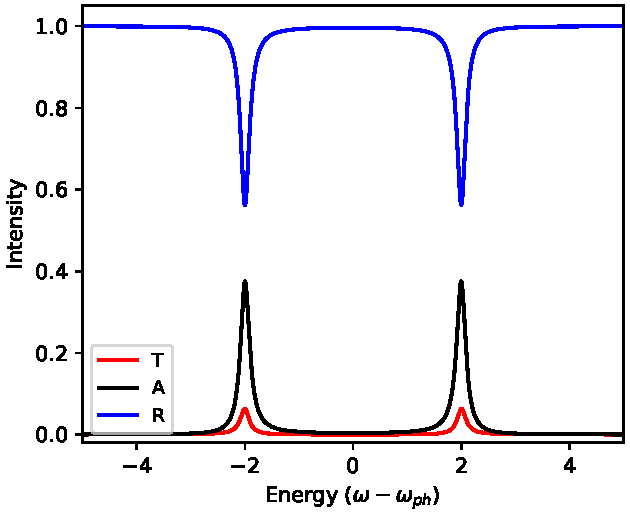
\includegraphics[width=\linewidth,height=0.60\textheight,keepaspectratio]
          {figures/linear_fig3a_reproduction.pdf}\\[-0.2em]
        $\omega-\omega_{\mathrm{ph}}$ {\scriptsize probe 相对于腔共振的频率失谐\par}
        \vspace{0.25em}}
    \end{column}
  \end{columns}
  \vspace{2.5em}
  {\centering\textbf{强耦合形成 LP/UP 两个本征模；
    弱 probe 扫描其本征频率，并在 $T/R/A$ 中读出双峰/双谷共振结构。}\par}
  \papersource{JCP 160, 154107 (2024), Eqs.~(37), (38), (40), Fig.~3(a).}
\end{frame}

\begin{frame}{二能级极化激元的布居与无序效应}
  \fontsize{7}{7.9}\selectfont
  \setlength{\abovedisplayskip}{1pt}
  \setlength{\belowdisplayskip}{1pt}
  \setlength{\abovedisplayshortskip}{0pt}
  \setlength{\belowdisplayshortskip}{0pt}
  \vspace{0.2em}
  \begin{columns}[T,onlytextwidth]
    \begin{column}{0.49\textwidth}
      {\centering
        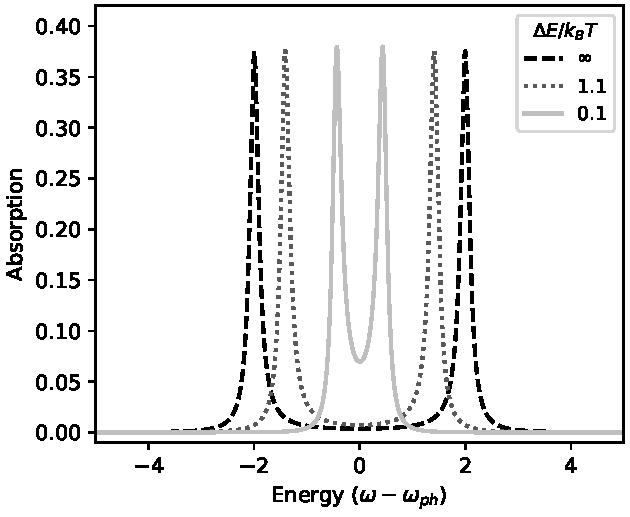
\includegraphics[width=\linewidth,height=0.52\textheight,keepaspectratio]
          {figures/linear_fig3b_reproduction.pdf}\par}
      {\scriptsize\color{gray}$G=2$，$\kappa=0.1$，$\gamma=0.3$，
        $\Delta E/(k_BT)=\infty,\,1.1,\,0.1$。\par}
      \[
        \physmark{NavyBlue}{p17pop}{
          p_g-p_e
          =
          \tanh\!\left(\frac{\Delta E}{2k_BT}\right)},
        \quad
        \chi_{\mathrm{2LS}}\propto
        \physmark{Plum}{p17split}{p_g-p_e}.
      \]
      布居差减小 $\rightarrow$ 分子线性响应减弱
      $\rightarrow$ Rabi 劈裂收缩。
    \end{column}
    \begin{column}{0.49\textwidth}
      {\centering
        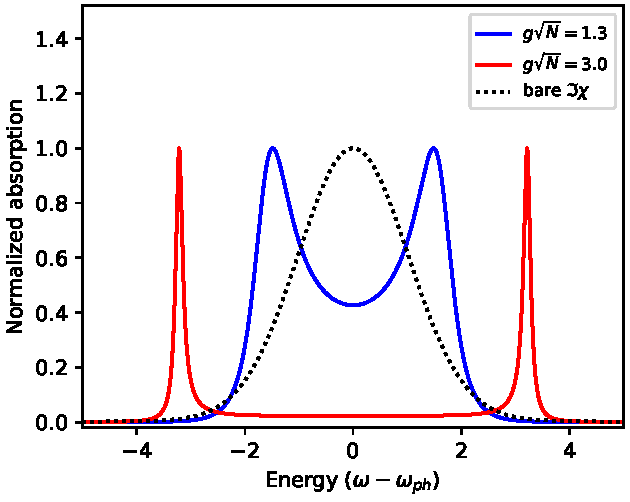
\includegraphics[width=\linewidth,height=0.52\textheight,keepaspectratio]
          {figures/linear_fig4c_reproduction.pdf}\par}
      {\scriptsize\color{gray}$\sigma=1$，$\kappa=\gamma=0.1$，
        比较 $G=1.3$ 与 $3.0$。\par}
      \[
        \physmark{NavyBlue}{p17sigma}{
          \omega_{\mathrm{exc}}
          \sim
          \mathcal N(\bar\omega,\sigma^2)},
        \quad
        \physmark{Plum}{p17ratio}{G/\sigma\uparrow}.
      \]
      当集体耦合超过非均匀展宽尺度时，
      极化激元线宽更多由均匀线宽与腔损耗决定。
    \end{column}
  \end{columns}
  \vspace{1.5em}
  {\centering\textbf{改变的都是分子侧 $\chi(\omega)$；
    上一页 $T/R/A$ 的通用形式保持不变。}\par}
  \papersource{JCP 160, 154107 (2024), Eqs.~(37), (41), (42), Figs.~3(b), 4(c).}
\end{frame}
